\section{Snedecor's $F$ Distribution}

The $F$-distribution is fundamental for comparing variances and in the Analysis of Variance (ANOVA).

\subsubsection{Definition}

\begin{definicion}[$F$-Distribution]
Let $\chi^2_{d_1}$ and $\chi^2_{d_2}$ be independent chi-square random variables with $d_1$ and $d_2$ degrees of freedom, respectively. The random variable
\begin{align}
 \label{eq:3.2.15}
 F = \frac{\chi^2_{d_1}/d_1}{\chi^2_{d_2}/d_2}
\end{align}
follows a \emph{Snedecor's $F$-distribution} with $(d_1, d_2)$ degrees of freedom. We write $F \sim F_{d_1, d_2}$.
\end{definicion}

{Properties}
\begin{itemize}
 \item $F \geq 0$ and the distribution is asymmetric (right-skewed).
 \item The probability density function of $F$ is
 \begin{align}
  \label{eq:3.2.16}
  f(x) = \frac{1}{B(d_1/2, d_2/2)} \left(\frac{d_1}{d_2}\right)^{d_1/2}
  x^{d_1/2 - 1} \left(1 + \frac{d_1}{d_2}x\right)^{-(d_1+d_2)/2},
  \end{align}
  where $B$ is the beta function.
 \item $E(F) = d_2/(d_2 - 2)$ for $d_2 > 2$.
 \item $\text{Var}(F) = \dfrac{2 d_2^2 (d_1 + d_2 - 2)}{d_1 (d_2 - 2)^2 (d_2 - 4)}$ for $d_2 > 4$.
 \item If $F \sim F_{d_1, d_2}$, then $1/F \sim F_{d_2, d_1}$.
\end{itemize}

\subsubsection{Application: Comparing Two Variances}

If $X_1, \ldots, X_{n_1} \sim N(\mu_1, \sigma_1^2)$ and $Y_1, \ldots, Y_{n_2} \sim N(\mu_2, \sigma_2^2)$ are independent samples, the ratio of sample variances
\begin{align}
 \label{eq:3.2.17}
 F = \frac{S_1^2/\sigma_1^2}{S_2^2/\sigma_2^2}
\end{align}
follows an $F_{n_1 - 1, n_2 - 1}$ distribution exactly (by Fisher's theorem applied to each sample). Under the null hypothesis $H_0: \sigma_1^2 = \sigma_2^2$, the statistic reduces to $F = S_1^2/S_2^2 \sim F_{n_1-1, n_2-1}$. This is the \emph{$F$-test for equality of variances}.

\begin{teorema}[Confidence interval for $\sigma_1^2/\sigma_2^2$]
 \label{eq:5.5.1}
With the notation above, a $(1-\alpha)\times 100\%$ confidence interval for the ratio of population variances is
\begin{align}
 \left[\frac{S_1^2}{S_2^2}\cdot\frac{1}{F_{n_1-1,n_2-1,\,\alpha/2}},\;\;
 \frac{S_1^2}{S_2^2}\cdot F_{n_2-1,n_1-1,\,\alpha/2}\right],
\end{align}
using the property $1/F_{d_1,d_2} \sim F_{d_2,d_1}$ to express the upper limit with a quantile of the "inverted" $F$.
\end{teorema}

\begin{observacion}[Connection to the $t$-distribution]
There is an elegant identity between $F$ and $t$: if $T \sim t_\nu$, then $T^2 \sim F_{1,\nu}$. This follows directly from the definitions: $T^2 = Z^2/(\chi^2_\nu/\nu)$, and $Z^2 \sim \chi^2_1$, so $T^2$ has exactly the form of a ratio of scaled chi-squared variables that defines $F_{1,\nu}$. This identity connects the three distributions studied in Sections 05.03--05.05: $\chi^2$, $t$, and $F$ are, at their core, different combinations of independent standardized normals.
\end{observacion}

\subsubsection{Application: ANOVA}

The Analysis of Variance (ANOVA) decomposes the total variability of data into components attributable to different factors.

\begin{teorema}[$F$-Statistic in ANOVA]
Consider $k$ groups with $n_i$ observations in the $i$-th group, and denote
\begin{align}
 \text{SS}_{\text{treat}} &= \sum_{i=1}^k n_i (\bar{X}_i - \bar{X})^2, \\
 \text{SS}_{\text{error}} &= \sum_{i=1}^k \sum_{j=1}^{n_i} (X_{ij} - \bar{X}_i)^2.
\end{align}
If $H_0: \mu_1 = \cdots = \mu_k$ is true, then
\begin{align}
 \label{eq:3.2.18}
 F = \frac{\text{SS}_{\text{treat}}/(k-1)}{\text{SS}_{\text{error}}/(n-k)} \sim F_{k-1, n-k},
\end{align}
where $n = \sum n_i$.
\end{teorema}

\begin{ejemplo}
 \label{exmp:3.2.6}
We want to compare the average performance of three teaching methods. The three methods are applied to groups of $5$ students each, obtaining the following scores:
\begin{align}
 \text{Method A: } 85, 90, 78, 92, 88 \quad (\bar{X}_A = 86.6), \\
 \text{Method B: } 79, 81, 85, 77, 83 \quad (\bar{X}_B = 81.0), \\
 \text{Method C: } 92, 95, 88, 90, 93 \quad (\bar{X}_C = 91.6).
\end{align}
Is there evidence that the methods produce different results?
\end{ejemplo}

\begin{solucion}
We calculate the variance components:
\begin{align}
 \bar{X} &= \frac{86.6 + 81.0 + 91.6}{3} = 86.4, \\
 \text{SS}_{\text{treat}} &= 5(86.6 - 86.4)^2 + 5(81.0 - 86.4)^2 + 5(91.6 - 86.4)^2 = 290.0, \\
 \text{SS}_{\text{error}} &= \text{within-group variance} \times (n - k).
\end{align}
To simplify, let us denote the sums of squares within each group. Calculating the deviations of each observation from its group mean:
\begin{align}
 \text{Method A: } & (85-86.6)^2 + (90-86.6)^2 + (78-86.6)^2 + (92-86.6)^2 + (88-86.6)^2 = 119.2, \\
 \text{Method B: } & (79-81)^2 + (81-81)^2 + (85-81)^2 + (77-81)^2 + (83-81)^2 = 40.0, \\
 \text{Method C: } & (92-91.6)^2 + (95-91.6)^2 + (88-91.6)^2 + (90-91.6)^2 + (93-91.6)^2 = 23.2, \\
 \text{SS}_{\text{error}} &= 119.2 + 40.0 + 23.2 = 182.4.
\end{align}

The $F$-statistic is
\begin{align}
 F = \frac{290.0/(3-1)}{182.4/(15-3)} = \frac{145.0}{15.2} \approx 9.54.
\end{align}

Under $H_0$, $F \sim F_{2, 12}$. The critical value at the $5\%$ level is $F_{0.05, 2, 12} = 3.89$. Since $9.54 > 3.89$, we reject $H_0$: there is evidence that at least one method produces different results.
\end{solucion}

\lstinputlisting[language=Python]{../code/distribuciones-muestreo/distF.py}

\begin{figure}
 \centering
 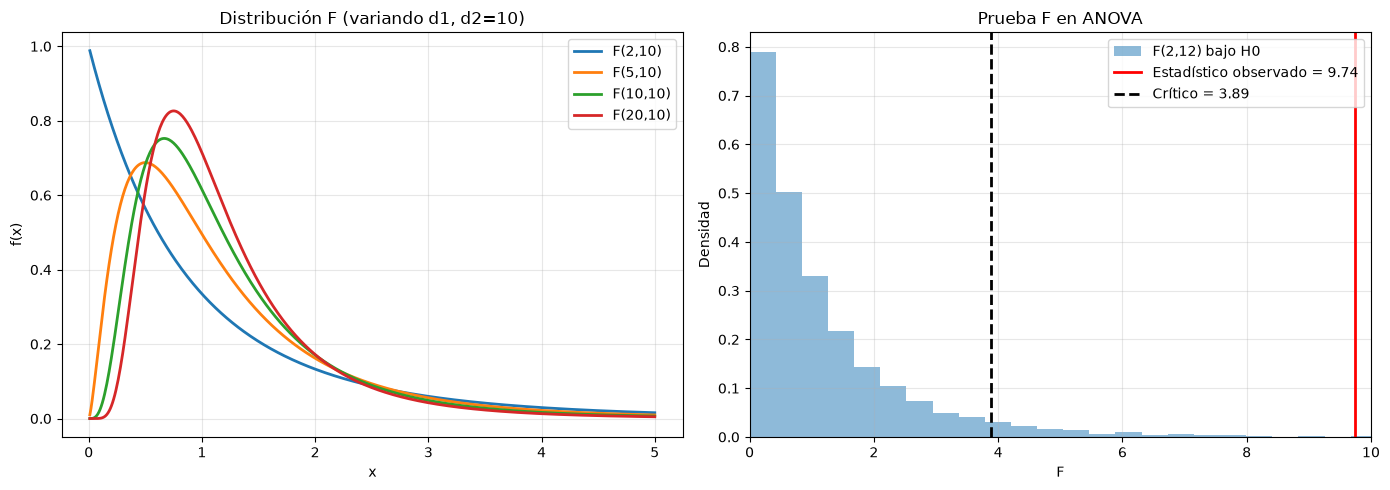
\includegraphics[height=7cm,keepaspectratio=true]{./pe/distF.png}
 % distF.png: 0x0 pixel, 300dpi, 0.00x0.00 cm, bb=
 \caption{Snedecor's $F$-distribution and application to ANOVA.}
 \label{fig:3.2.2}
\end{figure}
